\chapter{Demonstration of Baseline Compensation}
\textcolor{red}{基線長補償システムの性能評価をするために、KAAGRAのXアームキャビティを防振した。}

\section{Overview of KAGRA}
\subsection{Status of KAGRA}
KAGRA is a 3km laser interferometer, constructed in Kamioka, Gifu, Japan, and is now in its final commisioning phase. The KAGRA project はこれまでに2つの試験運転を経て、今はLIGOとVirgoとの第三次共同観測(O3)にむけたphaseにいる。Table\ref{tb:tb600}にKAGRAのphaseをまとめる。1つめの試験運転はinitial KAGRA (iKAGRA) と呼ばれる、2016年の3月から4月に行われた、3kmのMichelson interferometerの試験運転である。ことのとき、テストマスは低温ではなく常温ではなかったが、3kmの長期線干渉計を地下で可動させることを実証した。そして次に2つ目の試験運転である、basekine KAGRA (bKAGRA) とよばれる、低温鏡をつかったMicelson干渉計の試験運転である。この運転では低温干渉計を稼働させることを実証した。そして2019年12月現在、LIGOとVirgoとの第三次共同観測(O3)にむけて、低温鏡を使用した Fabry-Perot Michelson interferometer (FPMI)のコミッショニングをおこなっており、中性子連星合体を$1\,\mathrm{Mpc}$で観測できる感度まで向上させるノイズハンティングを行っている。

\begin{table}[h]
  \caption{Summary of the phasec of KAGRA. MI: Michelson Interferometer, FPMI: Fabry-Perot Michelson Interferometer, DRFPMI: Dual-Recycled Fabry-Perot Michelson Interferometer, RSE: resonant sideband extraction}
  \begin{tabular}{lllll}
    \toprule
    &iKAGRA& \begin{tabular}{l}bKAGRA\\Phase1\end{tabular} & \begin{tabular}{l}bKAGRA\\for O3\end{tabular}  & \begin{tabular}{l}bKAGRA\\(final)\end{tabular}  \\ \midrule
        
        \begin{tabular}{l}Year\end{tabular}& \begin{tabular}{l}2016\\Mar - Apr\end{tabular}&\begin{tabular}{l}2018\\Apr - May\end{tabular} & \begin{tabular}{l}2019\\Dec - \end{tabular} & \begin{tabular}{l}2020 -\\(planned)\end{tabular} \\
              \begin{tabular}{l}Configuration\end{tabular} & \begin{tabular}{l}MI\end{tabular} & \begin{tabular}{l}MI\end{tabular} & \begin{tabular}{l}FPMI\end{tabular} & \begin{tabular}{l}DRFPMI\\(RSE)\end{tabular}\\
                      
                      \begin{tabular}{l}Test mass\\temperature\end{tabular} & \begin{tabular}{l}room temp.\end{tabular}& \begin{tabular}{l}18K\\room temp.\end{tabular} & \begin{tabular}{l}18K\\room temp.\end{tabular}  & \begin{tabular}{l}22K\end{tabular}             \\ \bottomrule
  \end{tabular}
\end{table}

%% KAGRAの最終的な感度は、resonant sideband extraction thechnique をもちいた Dual-Recycled Fabry-Perot Michelson interferometer で達成される。KAGRAの設計感度をFig.\ref{img:img600}に示す。

%% \begin{figure}[h]
%%   \begin{center}   
%%     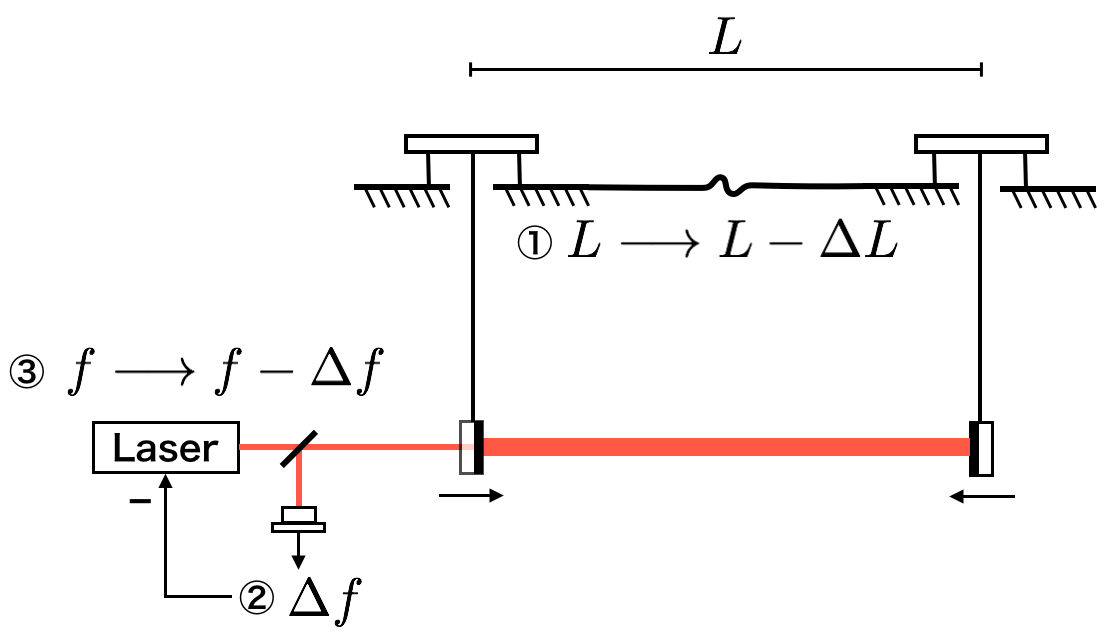
\includegraphics[width=12cm]{./img_chap6/img600.png}
%%     \caption{The designed sensitivity of KAAGRA \cite{akutsu2019first}}{}\label{img:img600}
%%   \end{center}
%% \end{figure}

\subsection{Main Interferometer}
KAGRAのメイン干渉計の図をFig.\ref{img:img601}に示す。KAGRAは他のLIGOやVirgoと同様に、腕にFabry-Perot光共振器とリサイクリング光共振器をもつマイケルソン干渉計である。ただし他とことなるのは、腕共振器の鏡は$22\,\mathrm{K}$まで冷却されていることである。この鏡にはサファイヤを使用している。なぜならば極低温下でも高いthermal conductivity と高いQ値を持ち、それぞれの特徴が熱レンズ効果と熱雑音を低減できるためである。またKAGRAその他の鏡はすべて常温のfused silica 鏡である。

\begin{figure}[p]
  \begin{minipage}{15cm}
    \begin{center}   
      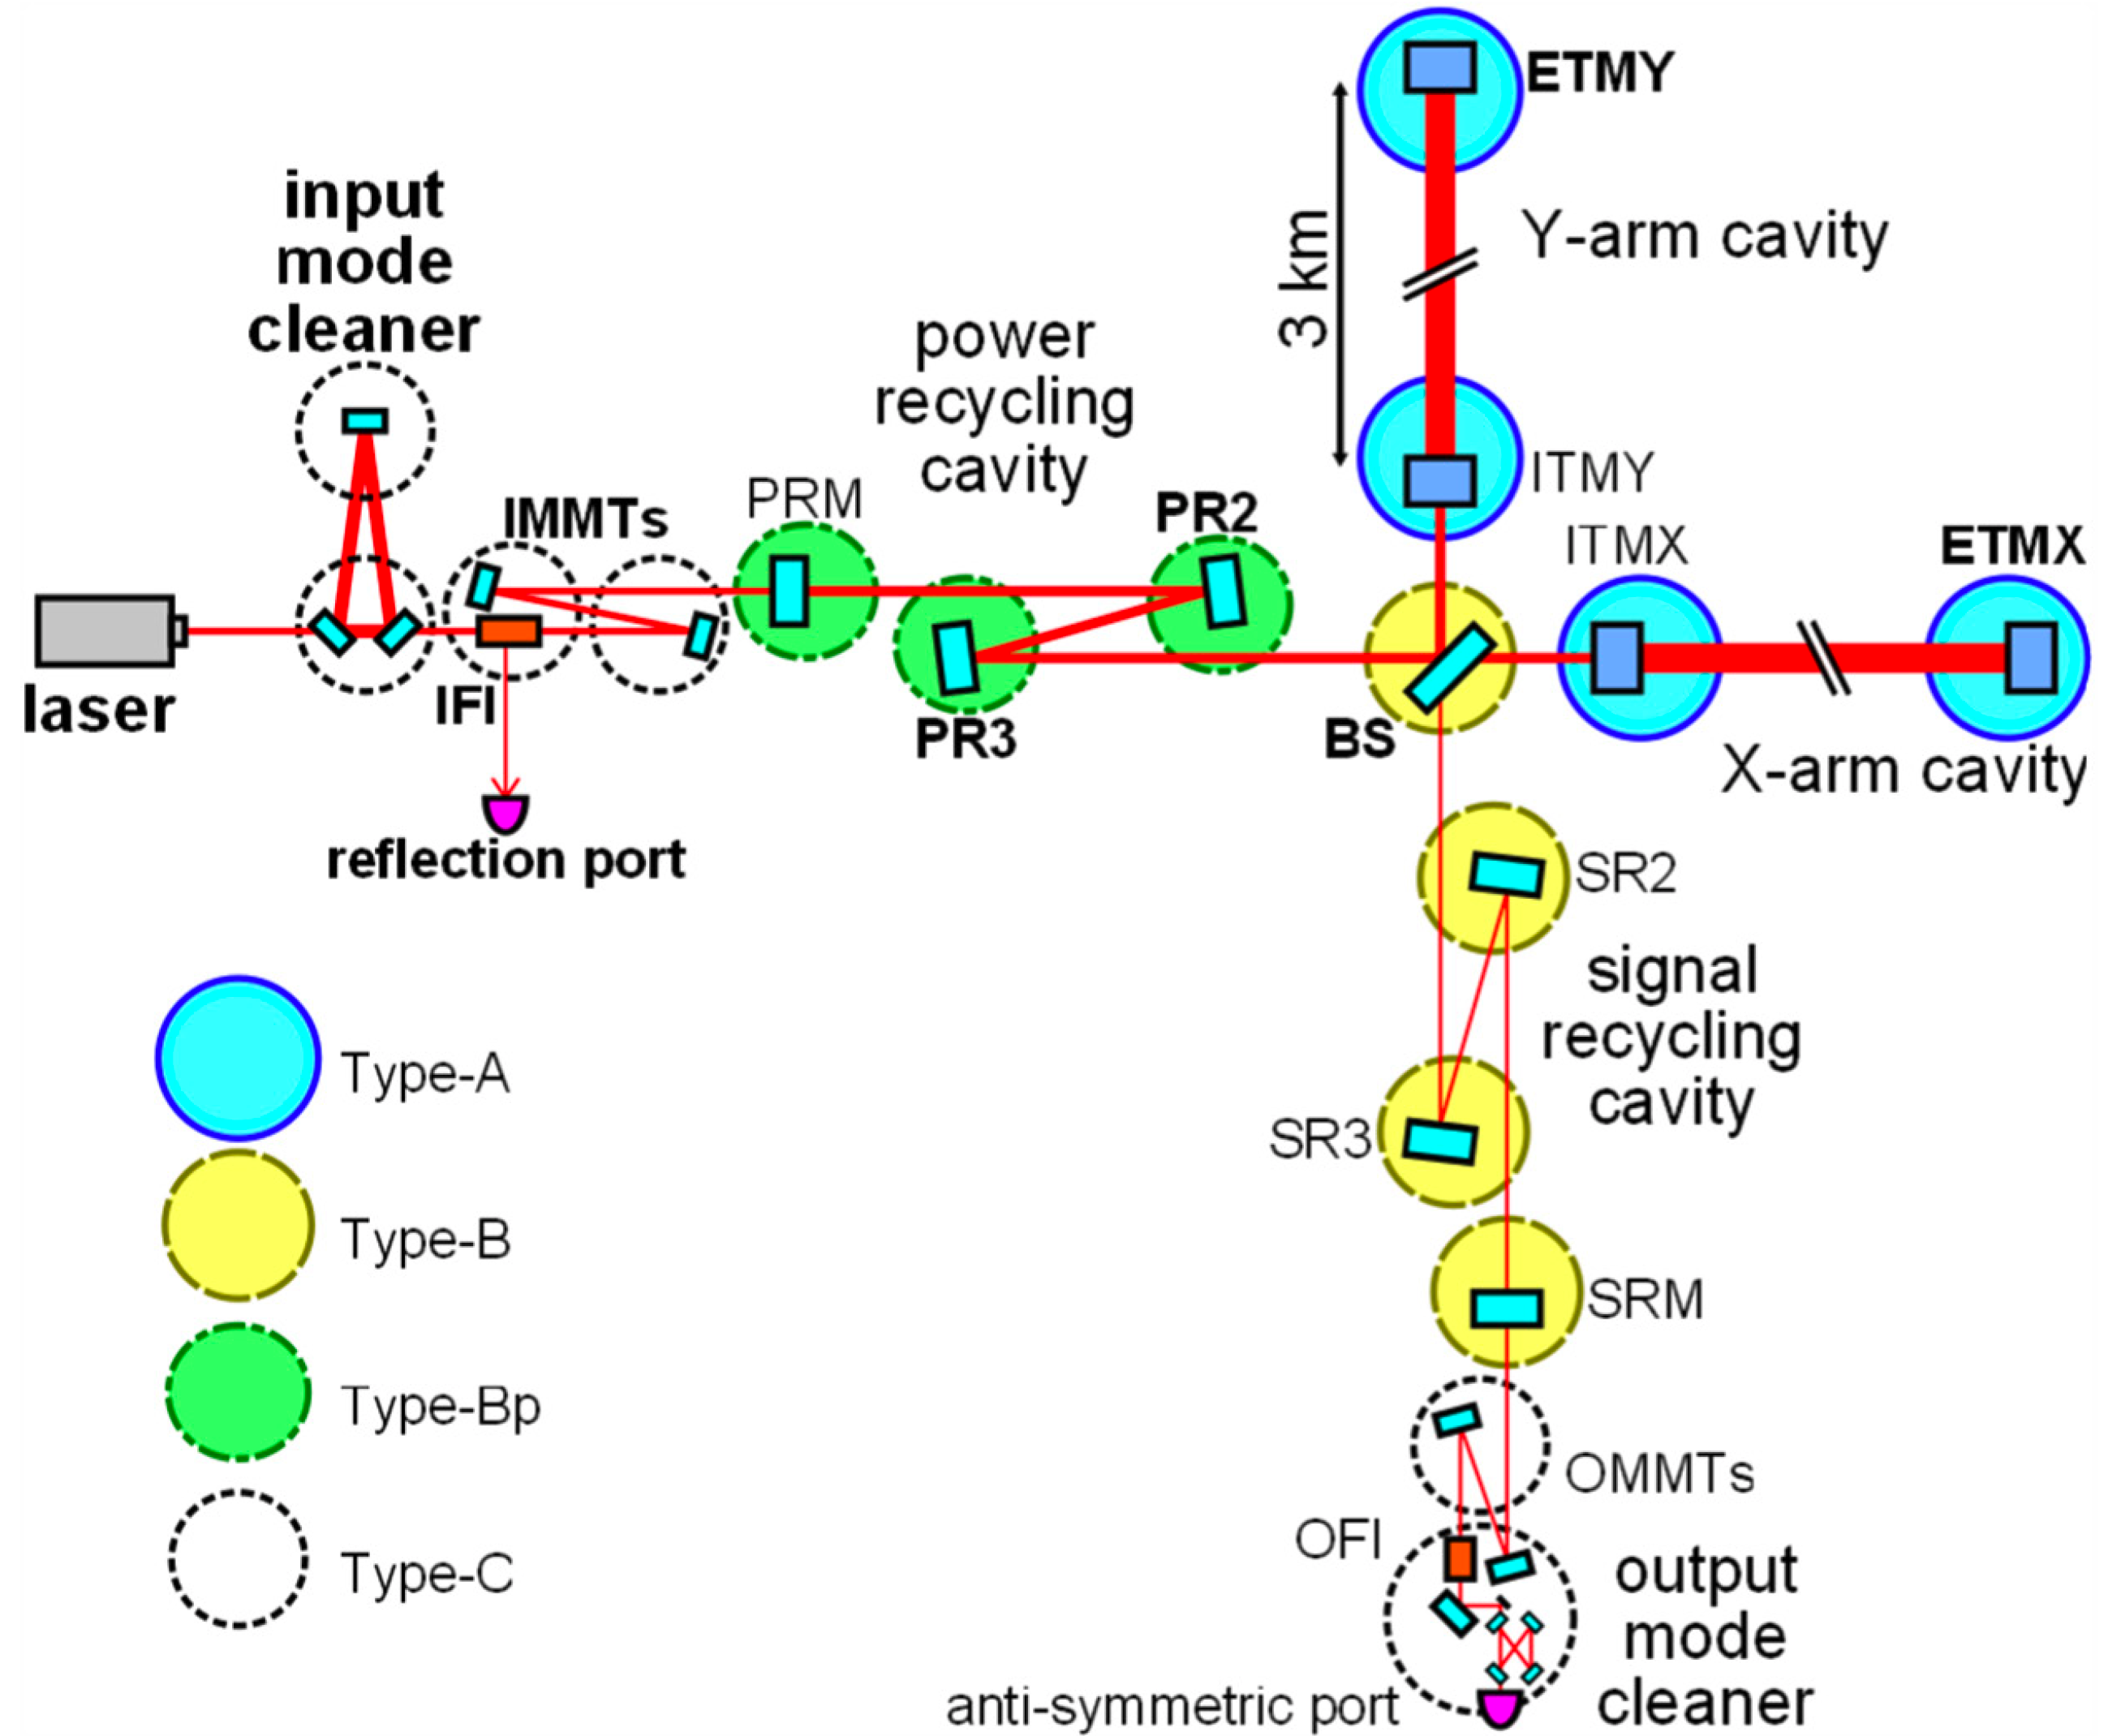
\includegraphics[width=13cm]{./img_chap6/img601.png}
      \subcaption{Schematic interferometer configuration of KAGRA \cite{akutsu2019first}}{}\label{img:img601} \hfill\vspace{10pt}
    \end{center}
  \end{minipage}
  \begin{minipage}{15cm}
    \begin{center}   
      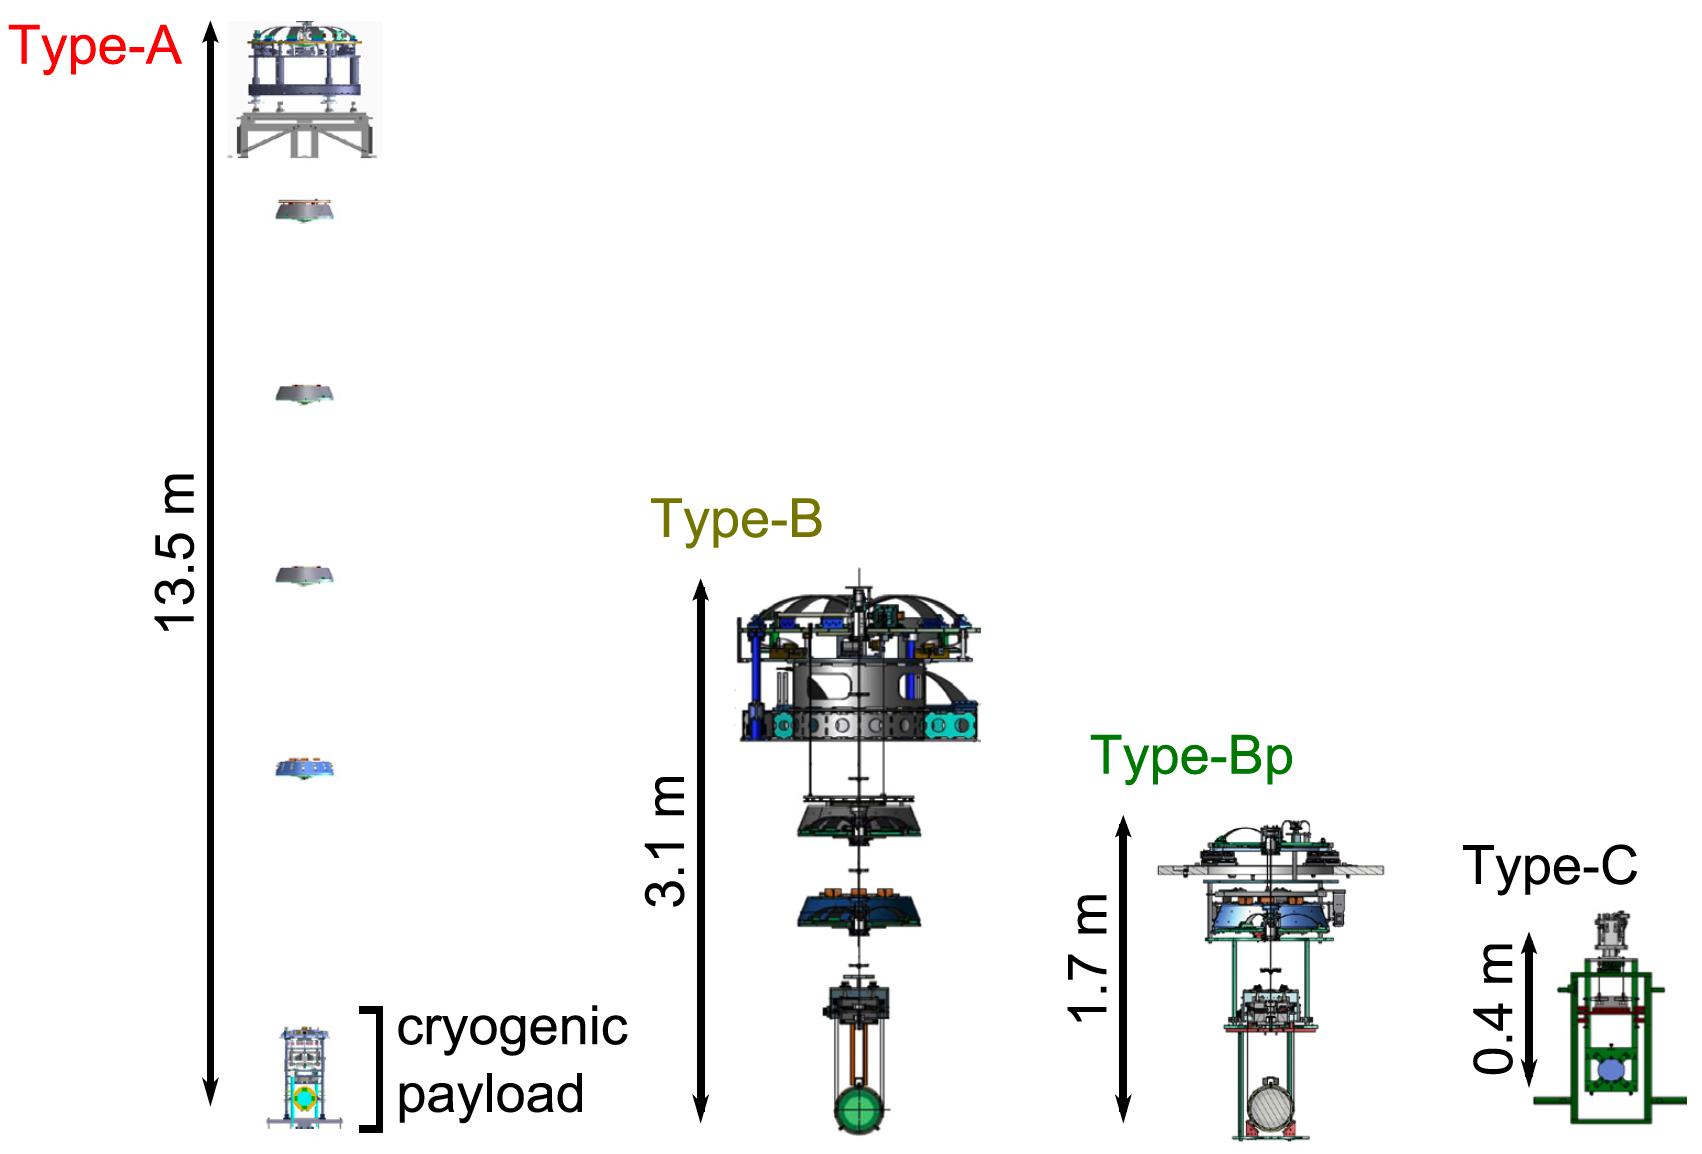
\includegraphics[width=13cm]{./img_chap6/img601b.png}
      \subcaption{KAGRA mirror suspension system \cite{akutsu2019first}}{}\label{img:img601b}
    \end{center}
  \end{minipage}
  \caption{Interferometer configuration and mirror suspension system}{}
\end{figure}


KAGRAの干渉計は、おもに4つに分けられる; arm caivties, input and output mode cleaners (IMC and OMC), power resycling cavities (PRC), and signal resycling cavities (SRC). Arm cavities are composed of input test masses (ITMs) and end test masses (ETMs). また低温鏡であるITM内部でのパワーをへらすために、フィネスは1530と他の検出器とくらべて高い。IMCは入射光の空間モードの整形と周波数を安定化させるために使われ、OMCは出射光のunwanted higher-order spatial modes とfrequency sideband を落とすためにある。IMCは3つの鏡で構成される三角共振器であり、およそ1Hz以上の周波数のpre-stabilizationができるように設計されている。またOMCは4つの鏡から構成されるbow-tie cavityである。PRC はBSと共振器をつくるPRMの他にPR2とPR3鏡で構成される。この共振器で入射光のパワーを10倍増幅させる。SRCはSRMとSR2、SR3で構成される。SRCは検出器を広帯域にして重力波信号を抜き出すために使われる。This technique is more important than Advanced LIGO and Advanced Virgo, because the bandwidth is narrower than other detectors due to a high finesse arm cavity of KAGRA. 

\subsection{Mirror Suspension System}
KAGRAの干渉計を構成する鏡はすべてSuspensionで懸架されており、それらは4つの種類がある; Type-A, Type-B, Type-Bp, Type-C. Type-Aはテストマス懸架するため、最も高い防振比が求められ、13.5mの9段振り子である。次に変位雑音への要求が高いシグナルリサイクリング鏡は、Type-Aの段数を減らした、Type-B Suspensionで懸架される。そしてType-Bpはさらにpre-isolatorを取り除いたSuspensionであり、Power rycycleを懸架している。最後に、Type-Cは最も簡易的な振り子でTAMAで使用されていたものを修正したSuspensionである。

\begin{figure}[p]
  \begin{center}   
    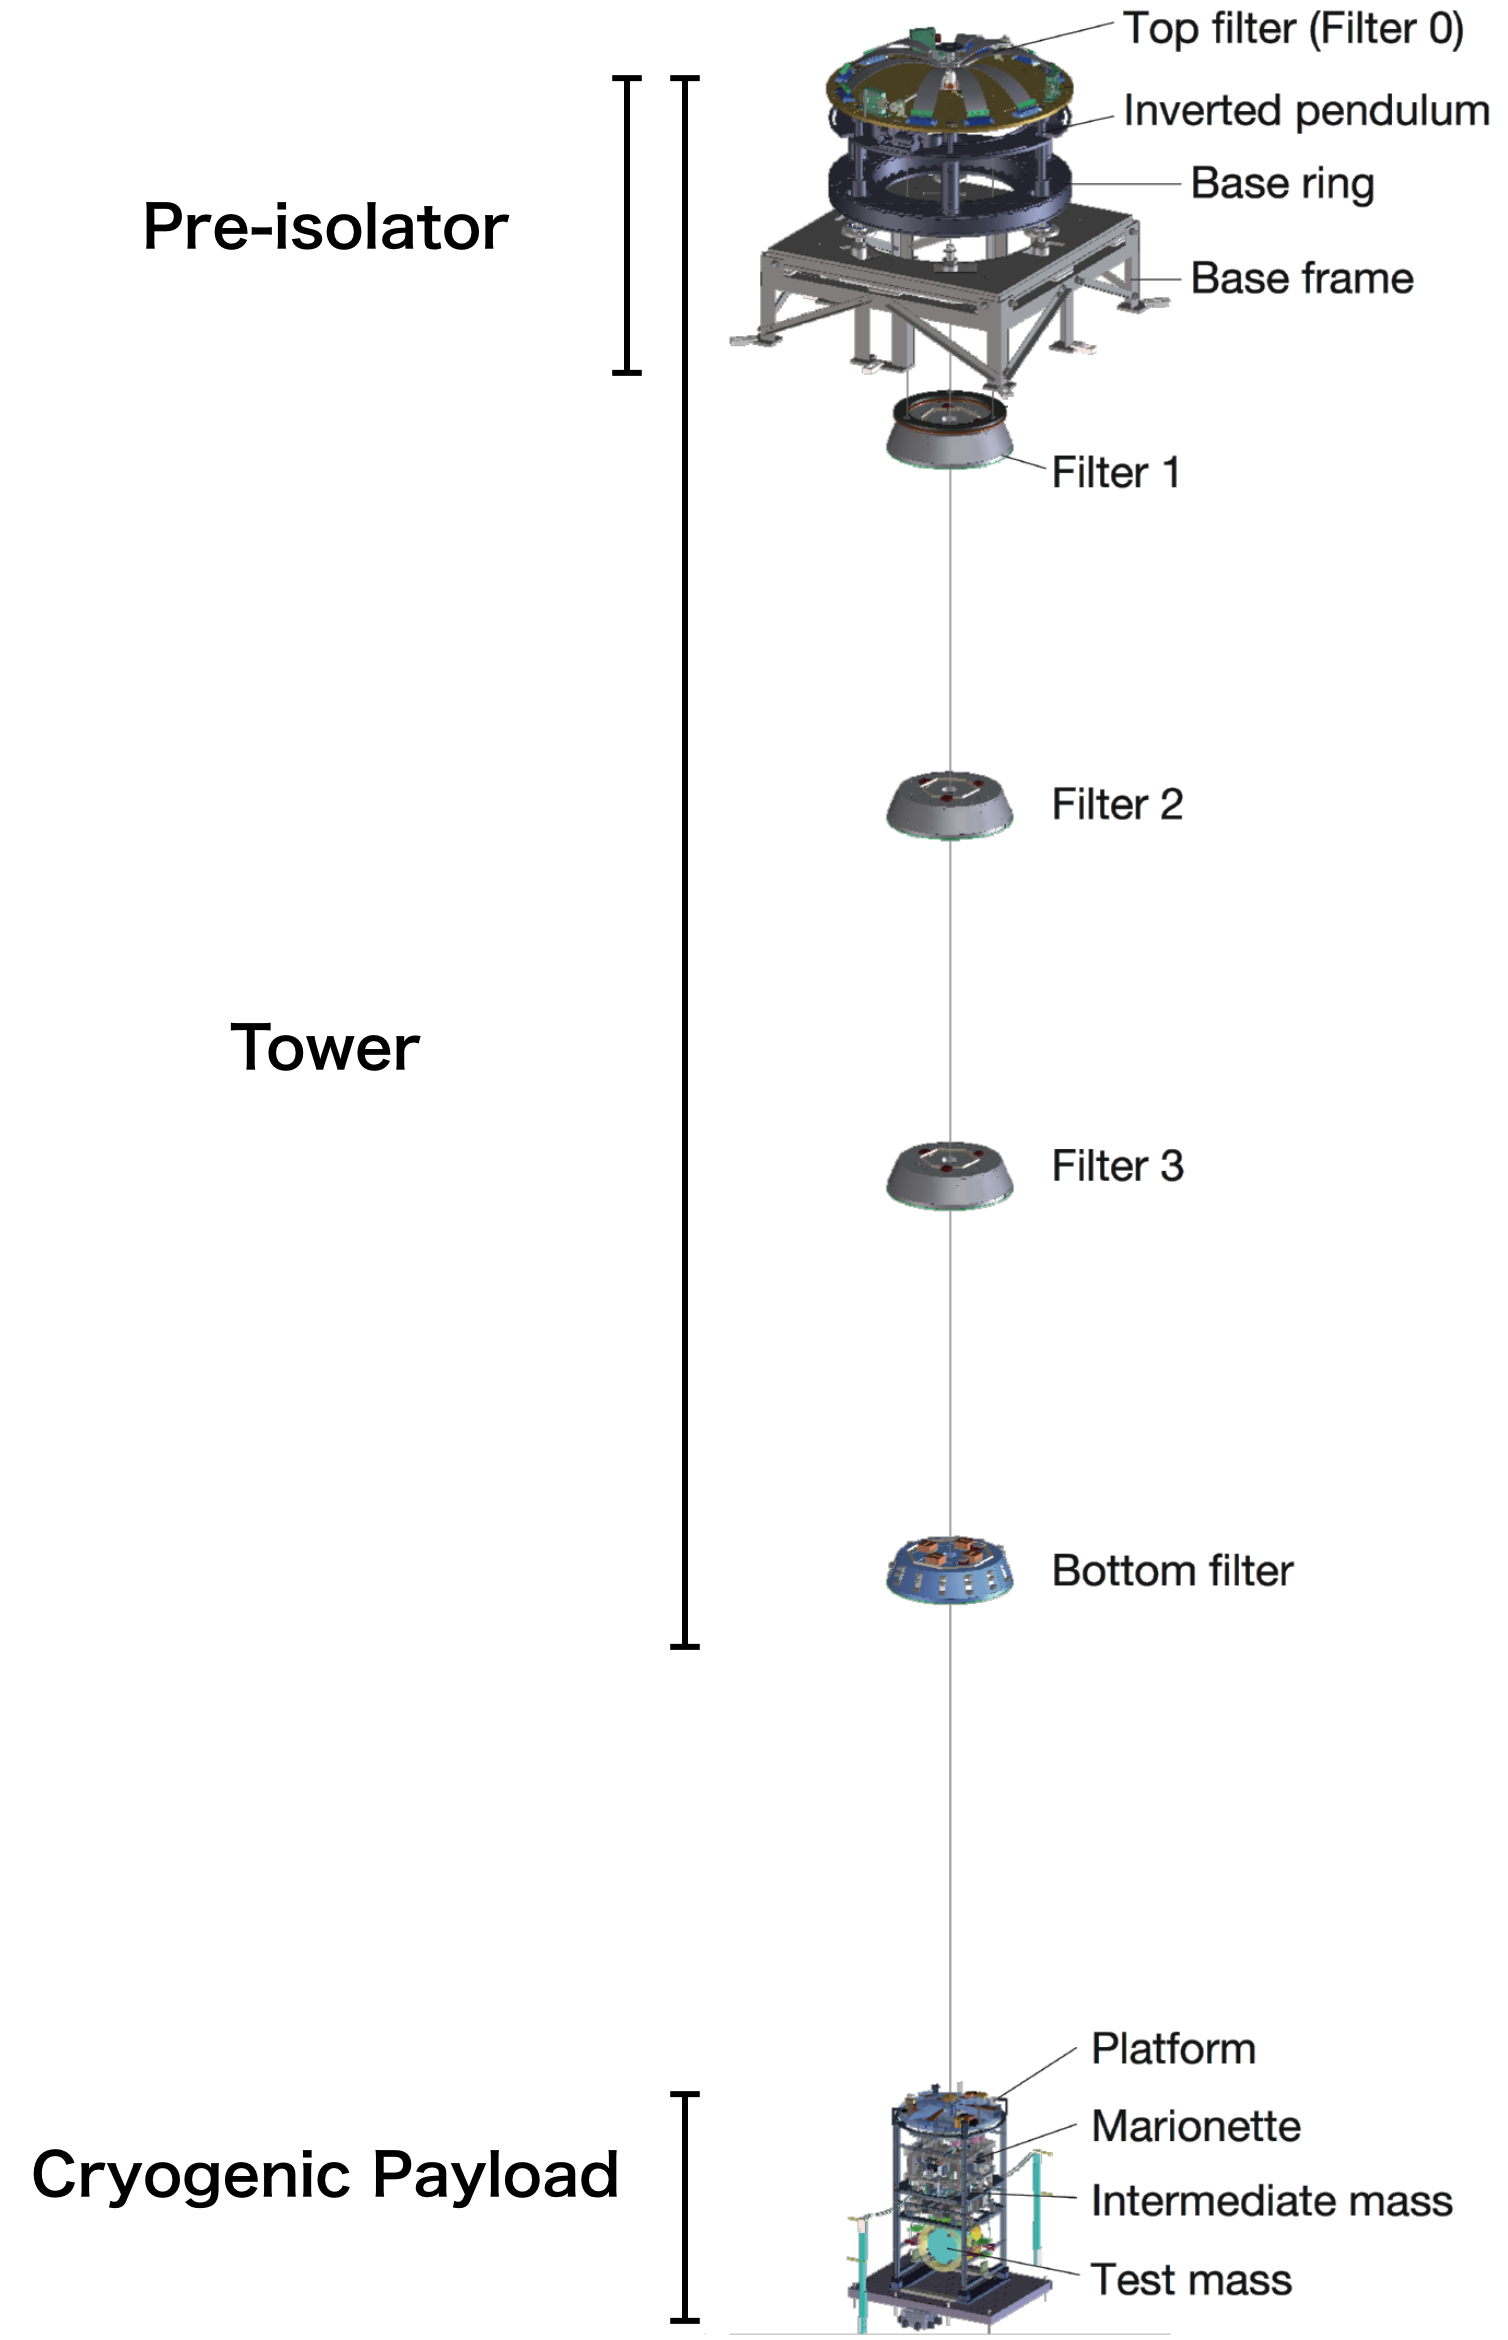
\includegraphics[width=13cm]{./img_chap6/img604.png}
    \caption{An overview of the Type-A suspension \cite{Okutomi2019development}. Test mass is suspend by a $13.5\,\mathrm{m}$ pendulum consisted of several mechanichal filters. The suspension point of the long pendulum is suported by the pre-isolator, which consists of inverted pendulum, on the ground through the base frame and base ring.}\label{img:img604}
  \end{center}
\end{figure}

\begin{figure}[p]
  \begin{minipage}{1.0\hsize}
    \begin{center}   
      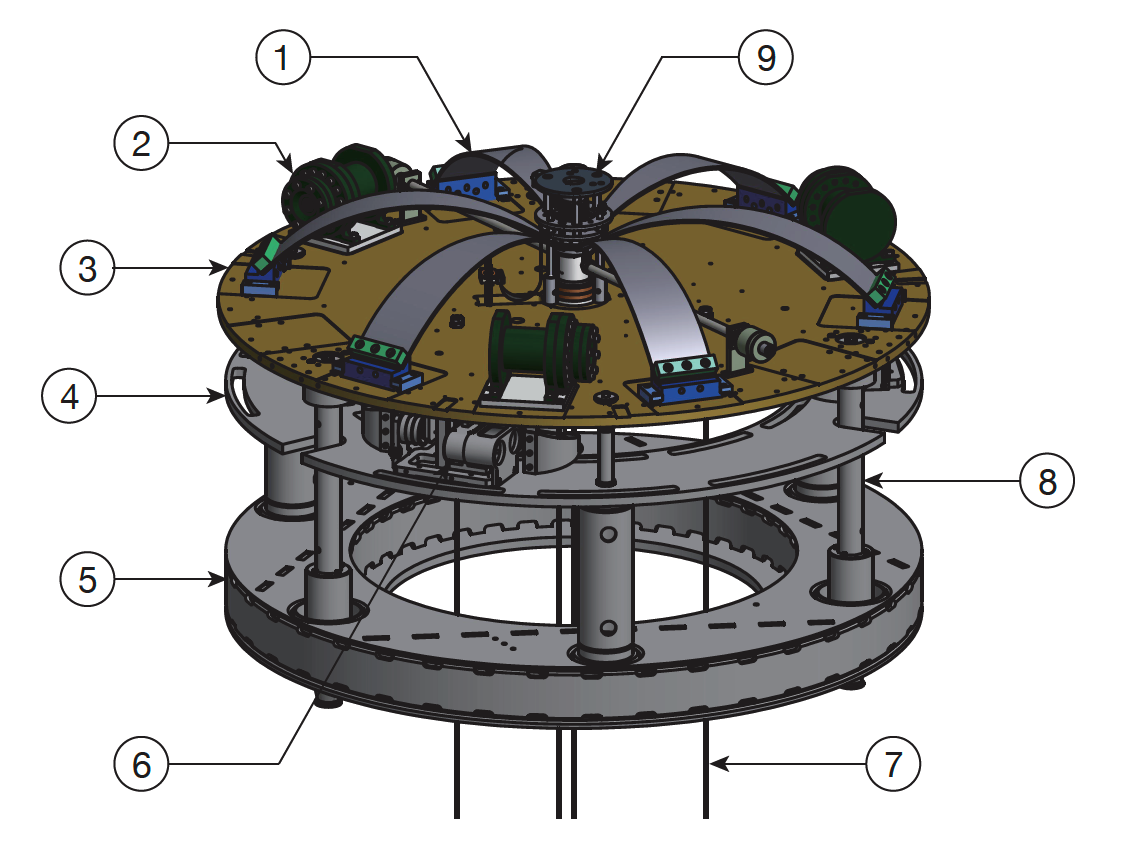
\includegraphics[width=12cm]{./img_chap6/img603a.png}
      \subcaption{Pre-isolator stage (PI). (1) Cantilever blade for GAS. (2) Geophone (3) Table of the top stage (4) Refernce frame rigidly connected to the base ring (5) The base ring mounted on the ground (6) LVDT and the coil magnet actuator (7) suspension wire to suspend the lower stages (8) leg of the inverted pendulum (IP). Figure is cited from figure 3.9 in \cite{Okutomi2019development}}\label{img:img603a}
    \end{center}
  \end{minipage}\\   
  \begin{minipage}[b]{0.5\hsize}
    \begin{center}
      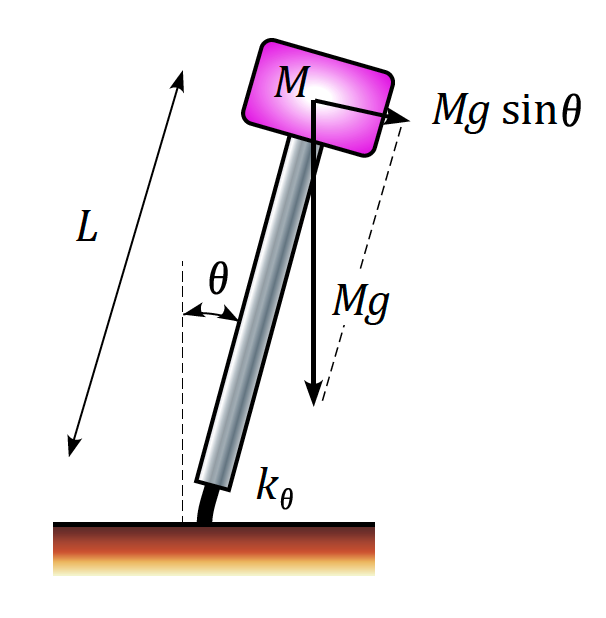
\includegraphics[width=8cm]{./img_chap6/img603b.png}
      \subcaption{Leg of the inverted pendulum (IP) \cite{sekiguchi2016astudy}.}\label{img:img603b}
    \end{center}
  \end{minipage}
  \begin{minipage}[b]{0.5\hsize}
    \begin{center}
      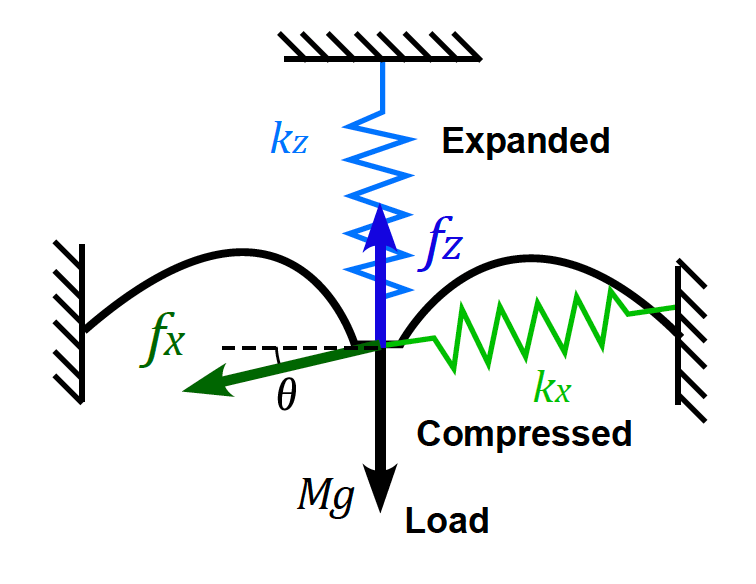
\includegraphics[width=8cm]{./img_chap6/img603c.png}
      \subcaption{Geometrical Anti-Spring \cite{sekiguchi2016astudy}.}\label{img:img603b}
    \end{center}
  \end{minipage}  
  \caption{CAD drawing of the pre-isolator (top) and main mechanical components of PI; IP leg and GAS (bottom).}
\end{figure}


\section{KAGRA Type-A Suspension}
\subsection{Overview}
In order to suspend the cryogenic test mass, as shown in Fig.\ref{img:img604}, KAGRA Type-A suspension has two parts; cryogenic payload and $13.5\,\mathrm{m}$ room temperature tower pendulum \cite{Okutomi2019development}. The cryogenic payload is consisted of Platform, Marionette, Intermediate mass, Test mass. The tower is consited of 5 mechanical filter; Top filter, F1, F2, F3, and Bottom filter. Moreover, the suspension point of tower is suspended by pre-isolator stage which has a inverted pendulum.

In terms of the low-frequency seismic attenuation, the pre-isolator is the important mechanical part.



\subsection{Pre-Isolator stage (PI)}
Pre-iolator(PI)は振り子の懸架点を防振するための能動防振システムであり、\cref{sec:sec}でのべた地震計と変位計をもちいた能動防振である。Fig.\ref{img:img603a}に示すように、機械的には、懸架点の並進方向はIvertedPendulumで、垂直方向はGASで防振されている。

\subsubsection{Inverted pendulum for horizontal vibration isolation}
Inverted pendulum はPreisolatorの荷重を調整することで、実質的なばね定数を小さくし、共振周波数を小さくすることができる。The angluar eigenfrequency of the singla IP leg is 
\begin{eqnarray}
  \omega_{\mathrm{IP}}=\sqrt{\frac{g}{L}\left(\frac{k_{\mathrm{\theta}}/gL-M}{M}\right)},\\
\end{eqnarray}
where is the bending spring constant of the flexure, $M$ is the mass of the stage and $L$ is the length of the leg. このように、原理上はステージの質量を調整すれば、共振周波数を0にすることができることがわかる。しかし、平方根の中がマイナスの場合振り子は不安定になるので、実際の共振周波数は$100\,\mathrm{mHz}$程度に設定されている。

\subsubsection{Geometric Anti-Spring for vertical vibration isolation}
GAS は向かい合わせたcantilever blades を圧縮することで、実質的な上下方向のばね定数を小さくする機械的なフィルターである。GASの固有周波数は、
\begin{eqnarray}
  \omega_{\mathrm{GAS}} = \sqrt{\frac{1}{M}\left[{ k_{z}- \left(\frac{l_{0}}{x_{0}}-1\right) k_{x}}\right]},
\end{eqnarray}
where $M$ is the load mass, $k_{\mathrm{x}}$ and $k_{\mathrm{z}}$ are the elastic constant of the compressed catilevers, $l_{0}$ is a natural length of the blades, $x_0$ is the horizontal distance between the central keystone and the support poit of the blades. One can find that the angular eigenfrequency of the GAS is reduced when $x_{0}<l_{0}$.

\subsubsection{Liner Variable Differential Transducer (LVDT)}
\begin{figure}[h]
  \begin{center}   
    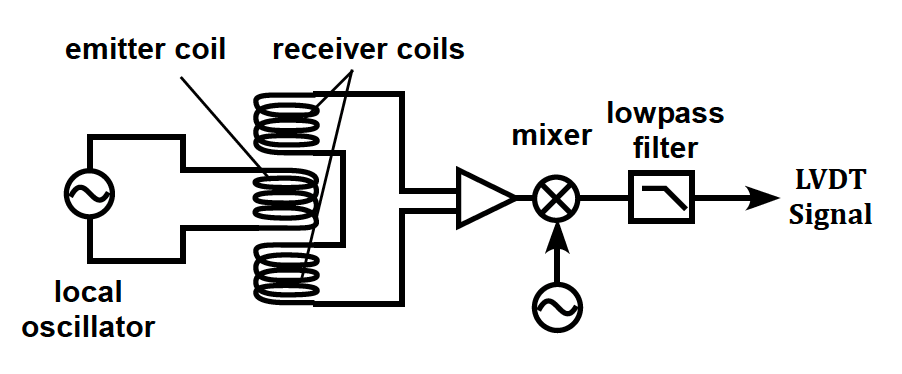
\includegraphics[width=10cm]{./img_chap6/img605.png}
    \caption{\cite{sekiguchi2016astudy}}\label{img:img605}
  \end{center}
\end{figure}
LVDT is a wide range relative position sensor composed of three coils \cite{Tariq2002hh}. shown in Fig.\ref{img:img605}. The emitter coil is mounted on the pre-isolator stage and driven with a sinusoidal signal to emit a modulated magnetic field. The two receiver coils is mounted on the reference structure, and these coils are counter-wound to each other. When the emitter coil is on the center of two reciever coils, induced voltage is not emitted from the reciever coils. On the other hand, when the pre-isolater is moved, a sinusoidal signal apprears on the reciever coils. Therefore, after demodulating this signal, amplitude of output signal is propotional to the displacement from the LVDT geometrical center.

\subsubsection{Coil-magnet actuator}
We use a voice-coil type wide range actuator to move the pre-isolator stage \cite{wang2002constant}.

\section{Experimental Arrangement}
\subsection{Length measurement of X-arm cavity}
腕共振器の長さ変化は、腕共振器が共振を維持できるように周波数アクチュエータであるAOMをつかって共振を維持した状態で、その制御信号からもとめた。



このとき、角度制御以外にマスアクチュエータを使っていない。


\subsection{Control Design}


\subsection{...}


\section{Results}
\subsection{Measurement Results}
\subsubsection{Reduction of the slow motion}
基線長補償システムをいれたときのXアーム共振器の腕の長さ変化をしらべた。Fig.\ref{img:img610}に、Xアームの制御信号とそのときの基線長伸縮を示す。12分に、補償システムをいれた。入れる前は、Xアームの長さは基線長伸縮によってゆっくりとドリフトしていたが、入れたあとは、そのドリフトはなくなっている。基線長はおよそ34分の間$8\,\mathrm{um}$ほど変化していたのに対して、補償システムをいれたあとはXアームの長さは$1\,\mathrm{um}$以下に低減されているので、およそ10分の1の低減が確認できる。

\subsubsection{Reduction in the microseismic region}
また、システムを入れる前後でRMS振幅場が小さくなっていることがわかる。システムを入れた前後の時系列データからもとめたASDをFig.\ref{img:img611}に示す。補償システムをいれたことで、0.01Hz以上の累積RMSの値が半分に減っていることがわかる。

\subsection{Comparison with the rigid body model}
Compare with the measured X-arm length fluctuation and the fluctuation estimated by the rigid body model of Type-A suspension. このモデルは、剛体モデルに基づいて力学の状態空間モデルを計算する\cite{sekiguchi2016astudy}。この状態空間モデルをつかって、地面振動からテストマスまでの伝達関数等を計算した。ただし、この伝達関数は振り子単体の伝達関数なので、ふたつの防振装置で防振される腕共振器を計算する場合、\cref{sec}で述べたように、CMRが十分大きい場合を仮定する。つまり、基線の地面振動の同相成分から腕共振器長変へのカップリングは無視できるものとする。

\subsubsection{When the compensation system is OFF}
補償システムがOFFのときのXアーム長変動の測定値と、そのときにモデルから期待されるものを比較する。Fig.\ref{img:img612}にその比較を示す。\cref{sec}で述べたように、補償システムを入れる前は、それぞれのPre-isolatorはそれぞれのローカルのLVDTをつかってFeedback制御されている。このときのLVDTのセンサーノイズを水色で、地面振動ノイズをオレンジ色で示す。これらノイズの二乗和のルートをTotalとし、赤色で示す。1Hz以上の、Xアーム測定の測定ノイズで埋もれている帯域を除けば、1Hz以下ではこのTotalは測定値と一致していることがわかる。

\subsubsection{When the compensation system is ON}
補償システムがONのときの比較をFig.\ref{img:img613}示す。ただし、we assumed the reduction factor of the sensor correction of 1./20 as mentioned in \cref{sec}. 補償システムがOFFになっていたときの比較では、1Hz以下でTotalと測定値が一致していたが、ONの場合では、予測されるTotalと測定値は一致していない。

\begin{figure}[p]
  \begin{minipage}{15cm}
    \begin{center}   
      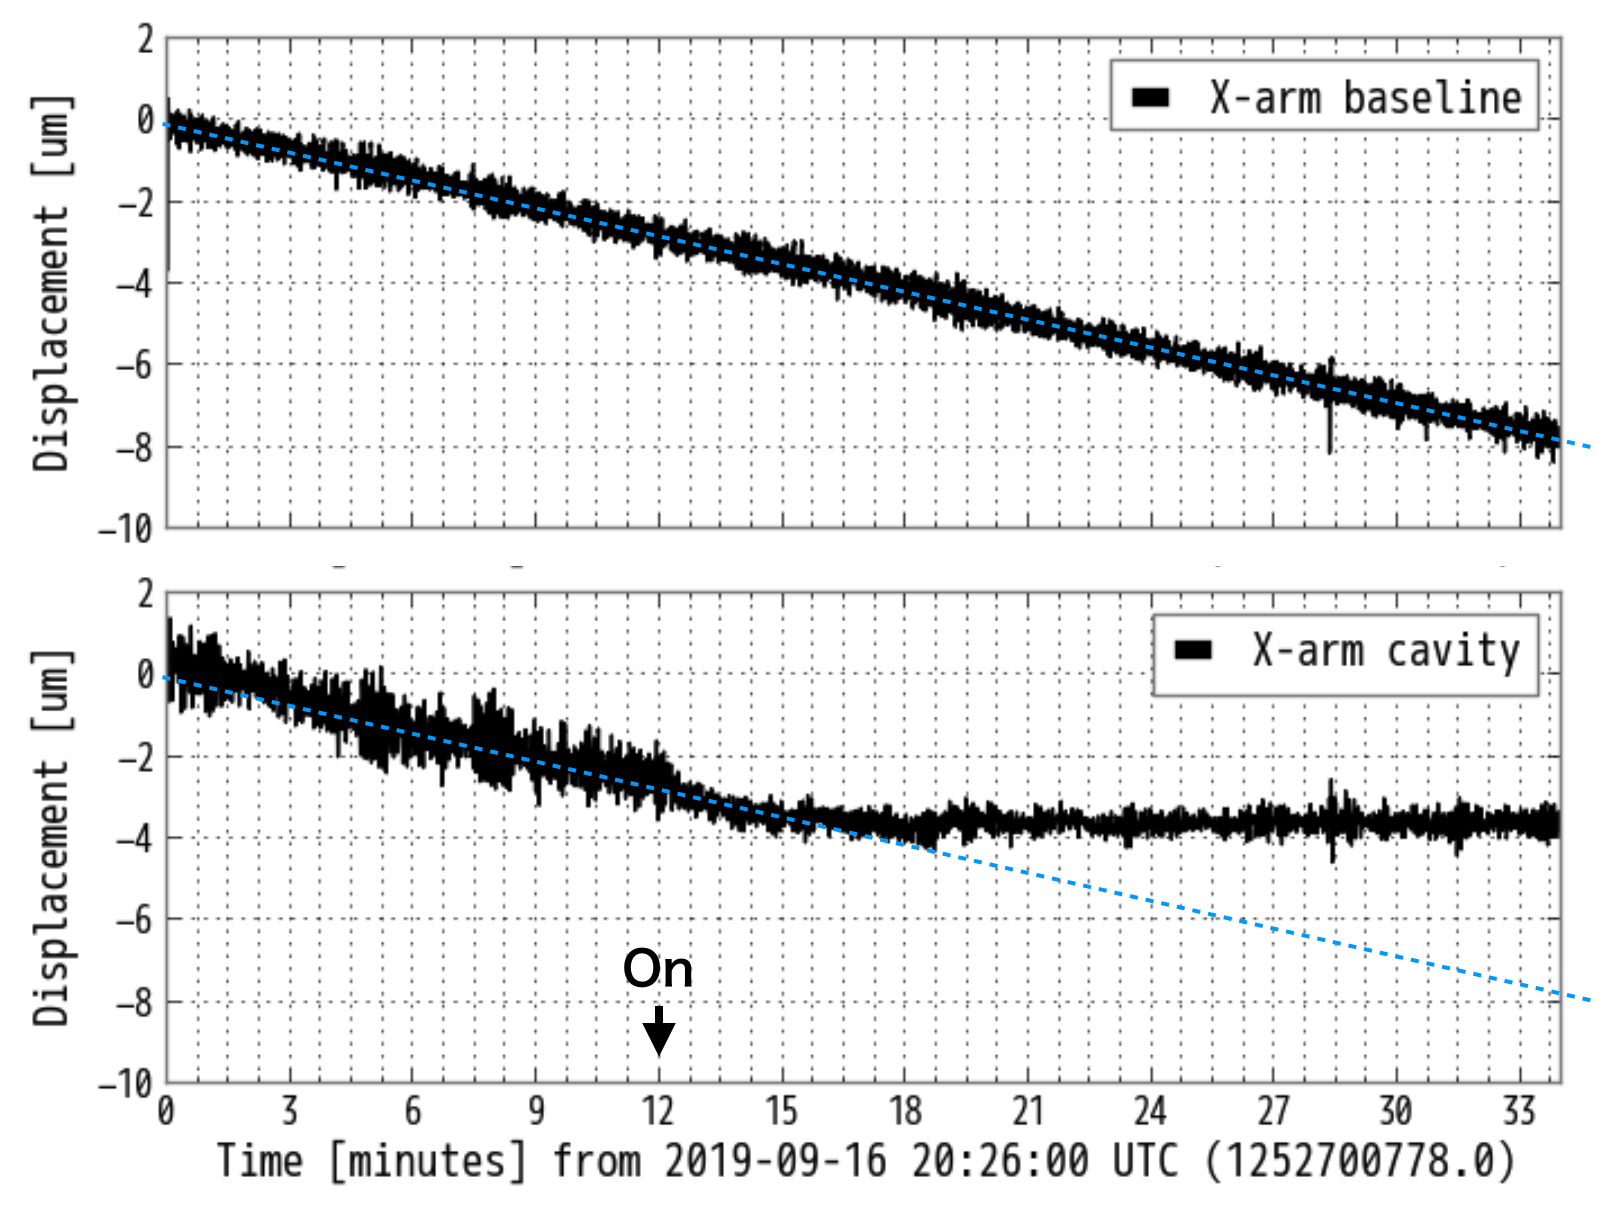
\includegraphics[width=12cm]{./img_chap6/img610.png}
      \subcaption{Length change of both X-arm baseline and X-arm cavity when baseline compensation system is turned on or off. At 12 minutes, the control is on.}\label{img:img610} \hfill\vspace{10pt}
    \end{center}
  \end{minipage}
  \begin{minipage}{15cm}
    \begin{center}   
      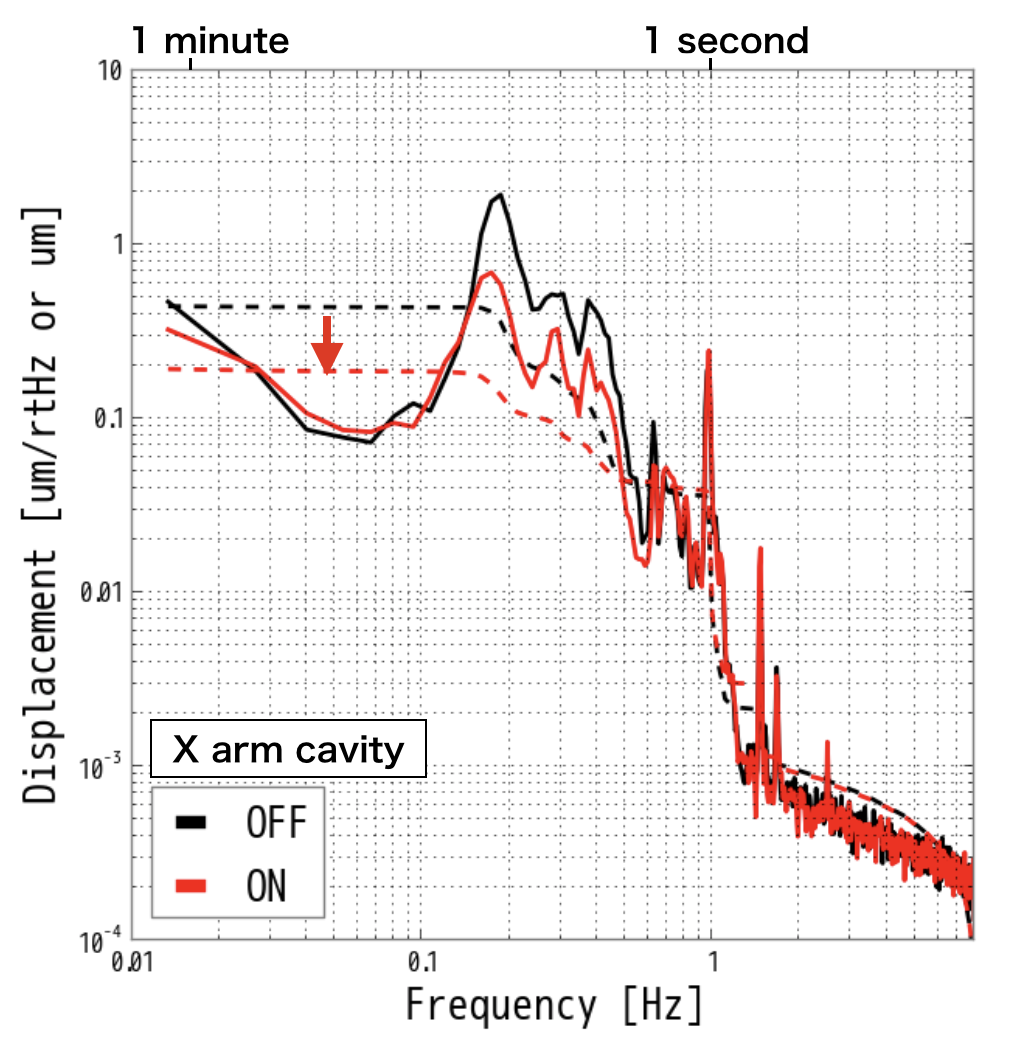
\includegraphics[width=10cm]{./img_chap6/img611.png}
      \subcaption{ASDs of X-arm caivty length when baseline compensation system is turned on and off. }\label{img:img611}
    \end{center}
  \end{minipage}
  \caption{Comparison of the reduction of the X-arm cavity length fluctuation when the baseline compensation system is turned on or off.}{}
\end{figure}




\begin{figure}[p]
  \begin{minipage}{15cm}
    \begin{center}   
      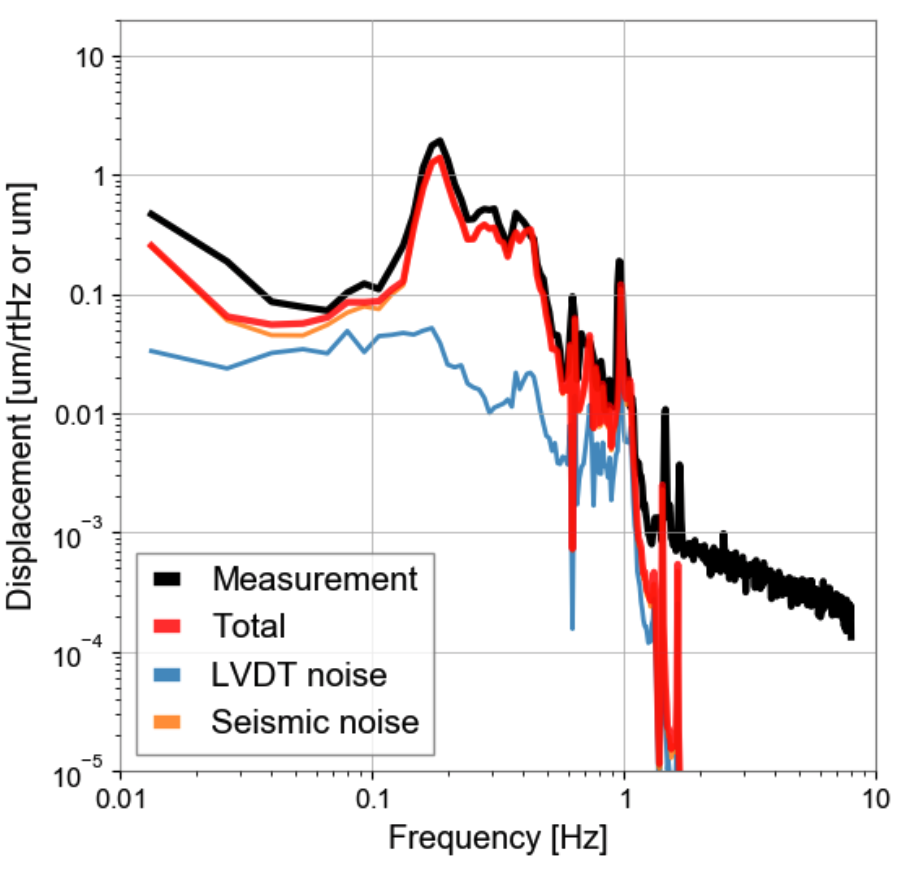
\includegraphics[width=9cm]{./img_chap6/img612.png}
      \subcaption{Noise budget of the X-arm length fluctuation when the compensation system is OFF. Measurement is same as the black line in Fig.\ref{img:img611}. Total is the summation of all noise contributions.}\label{img:img612} \hfill\vspace{10pt}
    \end{center}
  \end{minipage}
  \begin{minipage}{15cm}
    \begin{center}   
      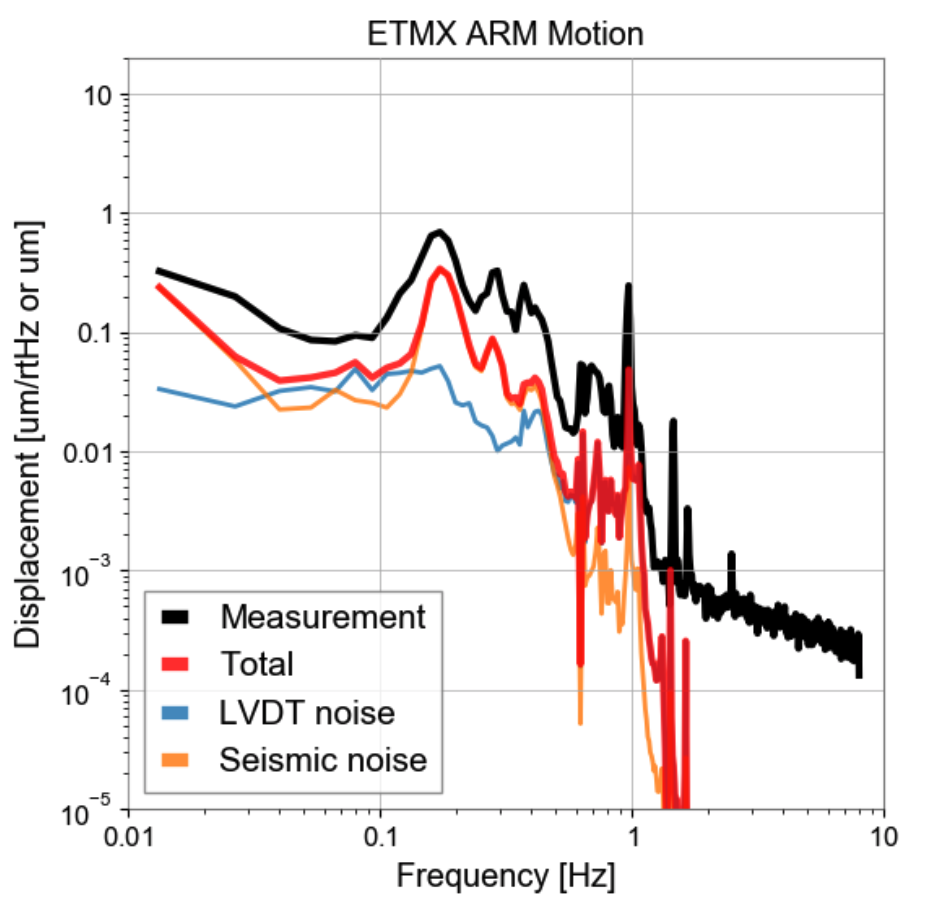
\includegraphics[width=9cm]{./img_chap6/img613.png}
      \subcaption{Noise budget of the X-arm length fluctuation when the compensation system is ON. Measurement is same as the red line in Fig.\ref{img:img611}. Total is the summation of all noise contributions assuming the reduction factor of sensor correction of 1/20.}\label{img:img613}
    \end{center}
  \end{minipage}
  \caption{Noise budget of the X-arm length fluctuation when the compensation system if turned on or off.}
\end{figure}



\section{Discussion and Summary of the Chapter}
\subsection{Discussion}
\subsection{Summary}
